\chapter{DATA}
\label{ch5:data}

The data used to test the hypothesis and aims introduced in the previous chapter are drawn from four clinical groups and  a set of simulated rs-fMRI sequences. In this chapter, we will first discuss the clinical images, which were taken from several prospective studies of congenital heart defects in pediatric patients as well as a prospective study of Alzheimer's disease in an aging population. Subjects from these studies were chosen because patient motion causes problems in MR images for the entire patient lifespan, though patients may exhibit different types of motion at different stages of life. 

Then we will discuss how we overcame the lack of objective ground truth in medical imaging research by developing a mechanism to simulate brain activity, scanner noise, and motion in rs-fMRI sequences.

\section{Clinical Cohorts}

The phrases congenital heart defects (CHDs) and congenital heart disease (CHD) both refer to defects in the heart or the vessels around the heart. CHDs affect how blood moves into, through, and away from the heart. 
CHD has a worldwide prevalence of about 8 per 1000 live births, meaning about 1.35 million children are born with CHD every year. %Since the survivability of CHD has increased from 10\% to 90\%, the medical community is faced with a growing, aging population of CHD patients. 

In this section, we provide a general overview of the impact of CHD on a global scale, the process for diagnosis, and additional risks associated with CHD. We then discuss the process of diagnosing neurodevelopmental comorbidities occurring with CHD and the impact of improved medical care on the CHD population. We end this section with a description of the four populations from which we obtained clinical rs-fMRI sequences.


\subsection{CHD Background}

\begin{figure}
\centering
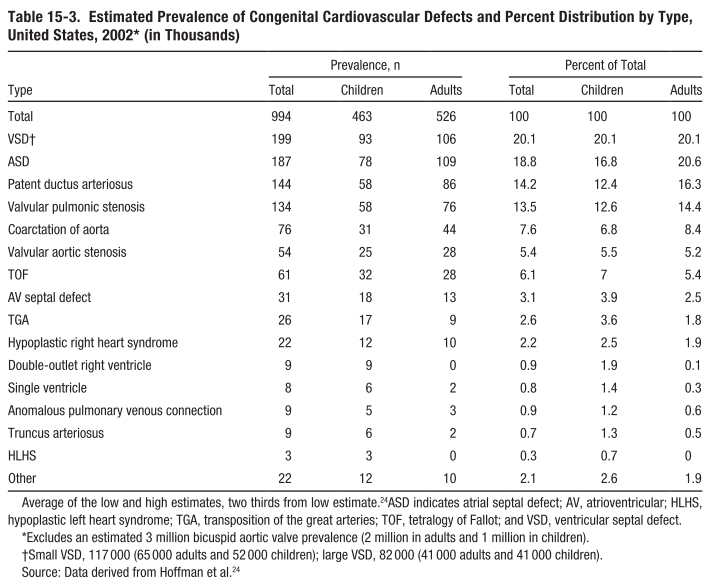
\includegraphics[width=0.6\textwidth]{5/chd-defects-usa.png}
\caption{Table of prevalences of congenital heart defects borrowed temporarily from \cite{Mozaffarian2016}.}
\label{ch5:fig:usa-defects-prev}
\end{figure}

CHD consists of a variety of defects which can affect any combination of the vessels and chambers of the heart with varying degrees of severity. The defects prevent the cardiopulmonary system as a whole from functioning correctly, but pinpointing and treating the defects effectively can be a complex process. It is important to note that each defect type has a different prevalence, a different treatment plan, and different expected outcomes. A breakdown of prevalence rates of some of the most common lesion types can be seen in Figure \ref{ch5:fig:usa-defects-prev}. % See (16)

% Causes of CHD: genetic syndromes, single gene mutations, environmental exposure, and unknown
Different presentations of CHD are associated with a number of different genetic and environmental factors \cite{Mozaffarian2016}. Genetic conditions such as Down syndrome, Turner syndrome, 22q11 deletion syndrome, Williams syndrome, and Noonan syndrome are associated with certain CHD presentations. Maternal behaviors such as smoking and binge drinking are known to cause heart problems in the fetus. Other maternal risk factors are obesity, folate deficiency, and living at a high altitude. Paternal exposure to phthalates, anesthesia, sympathomimetic medications, pesticides, and solvents may increase the risk of the fetus for developing CHD. While there are quite a few factors in this list, there are many CHD cases whose causes are unknown.

Once a patient is diagnosed with one of these defects or a cause of the CHD is identified, the specific nature of his case must be clearly documented. The documentation of CHD using the International Classification of Diseases, Ninth Revision, Clinical Modification (ICD-9-CM) has 25 high level codes representing various presentations of CHD, but these codes used alone are often not sufficient for describing a patient's true condition \cite{Mozaffarian2016}. Additional ICD-9-CM codes should be used to communicate the finer details of a patient's condition, if they are available. %something about how ICD codes make it easier to

The incidence of CHD in live births vary across countries and continents. The United States reports approximately 4-10 CHD case per 1000 live births. Europe and Asia see about 6.9 and 9.3 CHD cases per 1000 live births, though smaller studies have been conducted in many countries to measure local prevalence \cite{Mozaffarian2016}. In China, the incidence of CHD ranges from 8.98 to 11.1 per 1000 live births \cite{Zhao2019} \cite{Qu2016}. 
A pair of studies from Iran report incidences of 8.6 and 12.3 per 1000 live births, though the studies note that they were performed in different geographical locations with different populations within the country \cite{Nikyar2011} \cite{Rahim2008}.
One report from Dharan reports an incidence of 5.8 per 1000 patients admitted to a tertiary care hospital over a 12 month period \cite{Shah2008}. A study of newborns at one hospital in New Delhi, India claims an incidence of 3.9 per 1000 live births, though this rate may be a poor estimate as there is a significant delay between patient birth and referral to a cardiac center in India \cite{Khalil1994} \cite{Saxena2005}.

These incidence rates should be analyzed with some caution. In many cases, the reported rates were based on medical records. Medical records are not always correct; it is well known that human error can lead to a medical record lacking information or containing incorrect information. The only way for a person to have a medical record is for him or her to go to a medical center. Not everyone who has CHD is able to seek medical help, often because of their geographical locations or their income. Even if a patient is able to seek medical help, the availability of proper cardiac care varies between and within countries. However, it is generally expected that CHD incidence rates will increase as screening tools and treatments become more effective and more widespread, leading to earlier detection of defects.
 
% Diagnosis
Currently, the process of detecting and diagnosing CHD can begin before birth. A specialized ultrasound test called fetal echocardiography can detect heart abnormalities as early as the second trimester of the pregnancy. People who learn they are pregnant with a fetus who shows signs of CHD may choose to handle this information by opting for termination or pursuing a more detailed diagnosis. Additional tests, such as amniocentesis and follow-up ultrasounds may be used to determine treatment options before the patient is born. Generally, severe CHD cases present and are detected at earlier stages of life, but minor defects may not become apparent until the patient is older. Tests used to diagnose CHD in postnatal patients include electro- and echo-cardiograms, chest x-rays, pulse oximetry, exercise stress tests, computed tomography or MRI scans, and cardiac catheterization. Treatment of different defects varies from monitoring and medication to surgery and cardiac implants.

\begin{figure}
\centering
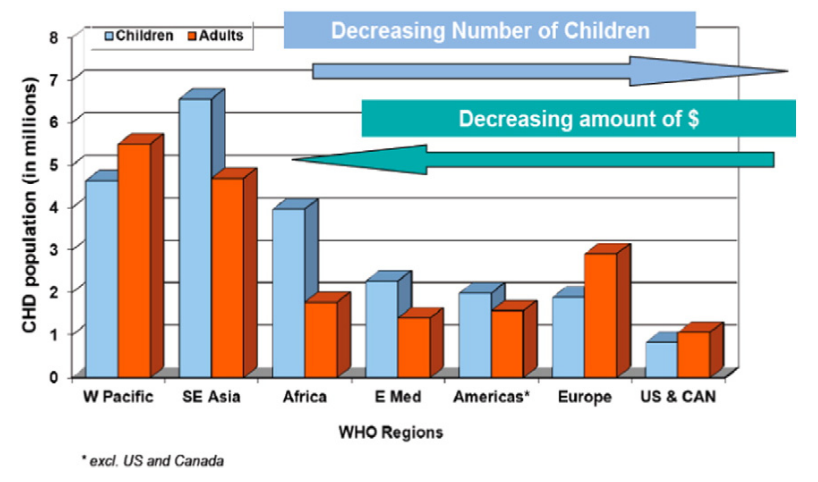
\includegraphics[width=0.7\textwidth]{5/CHD-burden-webb.png}
\caption{Estimated CHD burden in World Health Organization (WHO) regions using incidence rates of approximately 12/1000 and 4/1000 in children and adults, respectively \cite{Webb2015}.}
\label{ch5:fig:CHD-burden}
\end{figure}

%Depending on the cause of the 
The cost of diagnostic techniques and treatment plans impose different levels of financial burden on CHD patients and their families. Certain defects require complex, expensive surgical repairs while others can be treated with less expensive approaches \cite{Mozaffarian2016}. The burden of CHD across the globe was outlined by Webb et al \cite{Webb2015}. Their figure illustrating the prevalence of CHD and the availability of funds with which to treat it can be see in Figure \ref{ch5:fig:CHD-burden}. As the overall mortality of CHD declines, the burden of CHD is expected to increase \cite{Mozaffarian2016}.

% Complications and risks
Unfortunately, the cost of treating CHD is not the only burden a patient must undergo. Patients with CHD are also at increased risk for heart failure and infections \cite{Mozaffarian2016}. Children with CHD are at 19-fold risk for stroke compared to their healthy counterparts \cite{Fox2015}. In a study of Swedish citizens born between 1970 and 1993, Giang et al compared the prevalence of cardiac conditions in patients with and without CHD \cite{Giang2018}. They found that patients who had a CHD diagnosis were at about eight times higher risk for intracerebral hemorrhage and subarachnoid hemorrhage than their non-CHD counterparts. The CHD patients were also more likely to suffer from arrhythmia and heart failure. 

% When are patients diagnosed?
% Expected lifespan
% Treatment plan
% Financial burden

However, cardiac conditions are not the only complications CHD must deal with. Many of these patients also suffer from neurocognitive disorders that co-occur with CHD. Early research in this area focuses on the neurodevelopmental status of neonatal patients pre- and post-surgical intervention. One theory was that some factor or factors in the surgical intervention caused brain injuries in the patients. This idea proved to be inaccurate when researchers began detecting neurological malformations \textit{in utero}.

In a systematic review of available literature regarding prenatal and postnatal presurgical CHD cases and neurodevelopmental outcomes, Mebius et al. identify two theories about the causality of  neurodevelopmental delays and CHD \cite{Mebius2017}. The first theory is that abnormalities in the cardiac system prevent the developing brain from receiving enough oxygen and nutrients, which disrupts prenatal brain development. The second theory is that faulty genetic pathways used during both cardiac and brain development cause both conditions to co-occur. However, 11 articles Mebius et al. found during their review that are related to bloodflow through the umbilical artery suggest a third theory. During the prenatal period, a fetus receives oxygen from the mother via the placenta. If the placenta was not functioning correctly, it could lead to the fetus receiving not enough oxygen. Lower quantities of oxygen throughout prenatal development could potentially cause problems both in brain and cardiac growth. The 11 articles have contradictory results, but some researchers are currently investigating the role of the placenta in CHD and prenatal brain development.

Survival of CHD patients to adulthood has increased from 10\% to 90\% over the last several decades as CHD diagnostic tools and treatments have improved.  Currently, Webb et al. estimate that at least 12 to 34 million adults have CHD, and this number is expected to increase \cite{Webb2015}. The impact of the combination of CHD and neurological conditions throughout a patient's lifetime is starting to be explored. The aging of the CHD population has also sparked interest in the relationships between CHD and adult-stage neurological disorders such as dementia and Alzheimer's. 

While the purpose of this study is not to focus on CHD patients, we chose to use CHD and aging brain images in support of research being performed in the area of relationships between CHD and neurodevelopment.

%To address:
%\begin{itemize}
%\item Common combinations
%\item Joint treatment?
%\item Additional risks?
%\item Joint financial and emotional burden on caretakers? 
%\item CHD, neuro, and aging? Dementia/Alzheimer's? Recent data ... MIND neuroimaging ancillary r01 dec 17
%\end{itemize}


\subsection{Identifying Neurocognitive Disorders}

Neurocognitive disorders are usually diagnosed using at least one of many psychological survey-based evaluations, but these methods are subjective. rs-fMRIs could be used to identify patients who have functional connectivity patterns associated with different neurocognitive disorders, and eventually may be used to identify patients who are at risk for developing these disorders.

\subsubsection{Patient Surveys}

Surveys known to be used for studying the relationship between CHD and neurodevelopment are

\begin{itemize}
\item National Institute of Health Toolbox (3 - 85 years): ``Performance tests of cognitive, motor, and sensory function and self-reported measures of emotional function for adults and children in the general population and those living with a chronic condition''.

\item Sue Beers (4 - 18 years [not inclusive of 18 years]): WASI-II, NEPSY-2, WRAML-2, D-KEFS, WISC-IV, Grooved Pegboard, BRIEF, Beery-Buktenica VMI, ASRS, Conners-3, BASC-II, ABAS-II, PedsQL General, PedsQL Cardiac, Pictoral Scale Self Perception Profile.

\item SVR-III NDT (9 - 13 years [not inclusive of 13 years]): WIAT, NEPSY, WRAML, D-KEFS, WISC-V, Grooved Pegboard, BRIEF, Beery-Buktenica VMI, ASRS, Conners ADHD Index, BASC-II, ABAS-3, PedsQL General, PedsQL Cardiac

\item Bayley Scales of Infant and Toddler Development -III (1 - 24 months): Subtests include cognitive, language, social-emotional, motor, and adaptive behavior tests \cite{Mebius2017}.

\item Battelle Developmental Inventory (Birth - 8 years [not inclusive of 8 years]): Subsets include cognition, communication, social-emotional development, physical development, and adaptive behavior.

\item Developmental Assessment of Young Children (Birth - 6 years [not inclusive of 6 years]): Subtests include cognition, communication, social-emotional development, physical development, and adaptive behavior.

\item Preschool Language Scale + Receptive-Expressive Emergent Language (Birth - 3 years): Total language, auditory comprehension, expressive communication, articulation, receptive language, expressive language, and inventory of vocabulary words.

\item Peabody Developmental Motor Scales (Birth - 5 years): Subtests include reflexes, stationary, locomotion, object manipulation, grasping, visual-motor integration
\end{itemize}

The goal of these surveys is to compare the patient's cognitive function and neurological functions to expected milestones. Certain deviations from certain milestones are indicative of different disorders.

\subsection{Study Cohorts}

The rs-fMRIs used in this study were gathered as part of ongoing studies of the relationship between CHD and neurodevelopment as well as a national study of the aging brain. Data from the CHD/neurodevelopment studies was obtained through studies approved by the IRB at the Children's Hospital of Pittsburgh of UPMC and the University of Pittsburgh. Data from the again brain study was obtained from the Alzheimer's Disease Neuroimaging Initiative (ADNI) database (\href{adni.loni.usc.edu}{adni.loni.usc.edu}). All data is stored and accessed in compliance with HIPPA policies.

\subsubsection{Neonatal Cohort and Images}

Neonatal subjects have been recruited as part of a prospective observational study. The subjects were scanned using a 3T Skyra (Siemans AG, Erlangen, Germany). They were unsedated during the scans and a ``feed and bundle'' protocol was used to prevent motion during the scans \cite{Windram2011}. The newborns were positioned in the coil to minimize head tilting. Newborns were fitted with earplugs (Quiet Earplugs; Sperian Hearing Protection, San Diego, CA) and neonatal ear muffs (MiniMuffs; Natus, San Carlos, CA). An MR-compatible vital signs monitoring system (Veris, MEDRAD, Inc. Indianola, PA) was used to monitor neonatal vital signs. All scans were performed using a multi-channel head coil. The parameters for the resting-state BOLD MR scans were FOV=240 mm and TE/TR=32/2020 ms with interplane resolution of 4x4 mm, slice thickness of 4 mm, and 4 mm space between slices. The acquired images contained 150 volumes where each volume consisted of 64x64x32 voxels$^3$.

%\textbf{Neonatal Cohort.} Our set of neonatal subjects includes a cohort of 74 healthy neonates. Each subject in this cohort underwent an MRI scan, and the rs-fMRIs obtained during this process were compared to Power et al.'s positional and signal change usability thresholds. Of the 74 subjects, 17 of them had rs-fMRIs which did not meet the usability criteria. These high motion images were used to test the feasibility of the DAG-based volume registration framework. 

%Second, the neonates in this study were scanned using a feed and sleep protocol. Because the neonates were asleep during the scan, they generally did not move very much. The high-motion neonates are an obvious exception to this concept, but many of the high-motion images contained long periods where the subject was stationary. Evaluating the DAG-based framework on data with various patterns of motion and different periods of low and high motion allowed us to explore the effects of the DAG-based algorithm in different combinations of motion features. Third, these images were too corrupted by motion to be used in other analyses. 

%As the neonates were most often asleep during the scan, they exhibit less motion overall compared to our other clinical cohorts. Applying both the DAG-based framework and the traditional registration framework to these images provided the opportunity to compare the performances of both registration frameworks to each other in the context of the usability gold standard thresholds. 

%LEFT OFF HERE
The neonates were divided into CHD and non-CHD populations.

\subsubsection{Preadolescent Subject Population and Images}

As part of a multicenter study of CHD in preadolescents, we collected rs-fMRIs from nine sites throughout the United States. These images were of patients in the age range of 9 to 13 years who either had CHD or were healthy with no neurocognitive impairments. In addition to the MRI scans, subjects who participated in this study were asked to participate in additional testing  either to determine their neurocognitive outcome status or to perform genetic analyses. % (GET DETAILS FROM NANCY).

\textbf{Preadolescent Cohort.} The multicenter imaging study of preadolescent subjects provides a unique opportunity to evaluate the efficacy of the DAG-based framework on a large subject cohort containing variable amounts of motion. The outcome of this experiment will be used in the next experiment to determine if there are any site-specific or vendor-specific variables influencing patient motion.

%\begin{itemize}
%\item How were the images gathered?
%\item How were the patients recruited?
%\item What are the imaging protocol details?
%\item What other information was collected?
%\end{itemize}

\subsubsection{Fetal Subject Population and Images}

%Real goal is to develop a method of registering fetal brain and placental images so that we can further examine the relationship between placental oxygen levels and fetal brain development. Longitudinally, this technique can be used to determine how placental oxygen flow and fetal brain development impact a patient over the course of his or her life. Once the relationship between the placenta and fetal brain development is better understood, we can determine a set of neuroprotective interventions to employ for at-risk patients before they are born.

Fetal subjects have different constraints on their physical environment than neonates, preadolescents, and adults. As a result, they exhibit unique patterns of motion. The previous subject cohorts discussed in this chapter have the following commonalities: the subject experiences the full effects of gravity, the subject is lying on his back in an MRI scanner, and the subject's head motion is limited by the head coil within the MRI. Any motion in these images is a direct result of the subject himself moving, whether passively (cardiac motion and breathing) or actively (fidgeting or looking around).

A fetal subject is scanned in vivo. He is suspended in amniotic fluid within his mother. The amniotic fluid has buoyancy that reduces the effects of gravity and allows a fetal subject significant freedom of movement. The fetus can rotate, shift, and flip in ways that can only be accomplished when floating in a body of water. The properties of the uterus constrain the physical space in which a motion could occur, but not as much as the head coil and gravity do to the other patient cohorts. A fetus is not guaranteed to be in any specific position at the start of the scan: the scan begins when the mother is ready, not when the fetus achieves a certain pose. 

The fetal subjects underwent fetal echocardiography scans in a cardiac clinic to determine whether they were healthy or had a form of CHD. They were then scanned on an MRI scanner. Images of the fetal brain and the placenta were acquired for each subject. 

We are interested in both the fetal brain and placental images for our work because of the relationship between placenta and brain development. However, these organs have very different physical properties. The fetal brain is a rigid structure floating and moving within the amneotic fluid. It undergoes translation and rotation as a single unit due to passive and active maternal and fetal motions. The placenta, on the other hand, is anchored in place on the uterine wall. It may undergo small translations or rotations due to maternal motion, but it will respond differently to fetal motion. Fetal motions cause nonlinear deformations of the pliable placenta that can only be adequately accounted for using nonlinear registration algorithms. Nonlinear registrations have the potential to deform brain images into physically impossible shapes, so the fetal brain and placenta were manually segmented in their respective images so that each organ could undergo independent motion correction. 

The segmenters were one of a group of four researchers. While one researcher trained the other three group members, the interrater agreement between them is still being determined.

As the fetal subjects have both neurological and placental images, their data will be used to examine the impact of volume registration on different organ types.


%\begin{itemize}
%\item Fetal patients scanned between XX and XX weeks gestational age. 
%\item Imaging protocol details?
%\item What other information is collected about fetus and/or mom?
%\end{itemize}

\subsubsection{Aging Brain Subjects}

The ADNI study was launched in 2003 as a public-private partnership, led by Principal Investigator Michael W. Weiner, MD. The primary goal of ADNI has been to test whether serial magnetic resonance imaging (MRI), positron emission tomography (PET), other biological markers, and clinical and neuropsychological assessment can be combined to measure the progression of mild cognitive impairment (MCI) and early Alzheimer's disease (AD). For up-to-date information, see www.adni-info.org.

%\begin{itemize}
%\item How were the images gathered?
%\item How were the patients recruited?
%\item What are the imaging protocol details?
%\item What other information was collected?
%\end{itemize}

%The second adult cohort comes from the Alzheimer's Disease Neuroimaging Initiative (ADNI) dataset. The ADNI study has been working since 2004 to further Alzheimer's research by gathering, analyzing, and sharing clinical, imaging, genetic, and biochemical biomarkers from the elderly population. The group gathers data from 63 sites in the United States and Canada. During the second phase of the study, sites who have a Philips MRI system gathered resting-state fMRIs from their subjects. This data is freely available to academic researchers through the LONI Image and Data Archive.

The adult cohort encompass many clinical outcomes and a wider age range than the other clinical populations. The adult cohort also allows for another opportunity to study a different type of motion patterns associated with the aging brain rather than the still-developing brain.

\subsection{Summary}
%ELEPHANTS 3-5 sentences about CHD here

While we have amassed a large collection of clinical images, an analysis of purely clinical images is not sufficient in determining which volume registration technique recovers more brain signal. In the next section, we elaborate on this limitation and how we chose to address it.

\section{Simulated Sequences} % ELEPHANTS should this be its own chapter?

There are two major barriers in research surrounding motion correction in rs-fMRIs: gathering data and measuring the effects of the technique. 

It is difficult to obtain enough data from a large number of subjects to perform large-scale studies. Collaborators can band together to create a larger and more diverse data set by participating in multicenter studies. There are some challenges associated with multicenter studies. Each site will have a different scanner, potentially with different field strengths and from different manufacturers. Even ignoring the challenges of harmonizing data obtained using scanners from different companies, each scanner has its own set of unique inhomogeneities in the primary magnetic field. Additional scans of inanimate or human phantoms may be necessary to characterize the differences between all of the scanners involved.

The second barrier to motion correction in rs-fMRI research is the complexity of identifying a gold standard metric to use when evaluating motion correction techniques. The current gold standard metrics developed by Power et al. evaluate motion correction techniques in terms of the reduction of positional differences and signal differences between neighboring volumes. Unfortunately, this approach does not measure the amount of signal recovered or lost though motion correction. A true gold standard evaluation of motion correction would be able to evaluate the BOLD signal present in the image before and after correction. If the BOLD signal prior to patient motion was known, though, there would be no need for image processing in the first place: we would already have the data we are trying to obtain with motion correction.

We address these two barriers by creating a mechanism for generating simulated image sequences. The generated sequences contain simulated brain signal based in areas of the brain associated with resting-state connectivity, scanner noise, and patient motion. Our mechanism can create large quantities of unique image sequences. The simulated image sequences can also serve as a gold standard for evaluating volume registration and motion correction techniques: the signals and noise sources added to the sequence are known with certainty.

%Every MRI scanner is different, even those made by the same manufacturer. To ensure MRI scans obtained from different scanners are comparable.  so a stand-in model for an organ or tissue type is often used to calibrate an MRI scanner. The model is designed to have specific physical properties which mimic the physical properties of the organ or tissue. These properties can be accurately measured during the design process of this model so that the radiologist or researcher looking at images of the model can know the ground truth of the model. Because these models mimic true organs and tissues, they are called phantoms. 

\subsection{SPECTr: Simulated Phantom Emulating Cranial Transformations}

Our mechanism is called Simulated Phantom Emulating Cranial Transformations (SPECTr). A phantom is an object designed to have material properties which mimic those of a specific tissue type or organ. Phantoms, either manufactured objects or healthy humans, are used in multicenter studies to obtain images of the same object or person from multiple scanners. These images are used to harmonize the data taken from the different sites. We call our simulated sequence a phantom because the baseline image itself is known as are the signals added to it to simulate brain activity. 

% ELEPHANTS
When developing the pipeline for SPECTr, it was important to consider the effects of motion and various impacts they have on the BOLD signal. As discussed in CHAPTER, the three effects of motion are positional, spin history, and susceptibility. For simplicity, we combine the spin history and susceptibility effects into ...

\subsubsection{Materials}

In order to simulate resting-state BOLD signal in an fMRI, two pieces of anatomical information are required. The first is structural information about the brain. The second is the location of functional networks associated with the resting-state BOLD signal.

While it is possible to use clinical images for the structural information, the goal of SPECTr is to be generalizable both for our use and for the use of other researchers. Additionally, clinical images inherently contain some degree of signal from some neuronal processes which could obfuscate the simulated BOLD signal. 

In 1992, the International Consortium for Brain Mapping was formed to develop as set of standards for what is considered a healthy human brain. They used their criteria to develop an initial set of ``average'' brain structural scans based on scans from XXX healthy volunteers. This original set of average brain scans is referred to as the XXX brain. As MRI technology has improved, the scanners used to obtain the images of the healthy volunteers have become outdated. In XXXX, another set of healthy volunteers was recruited to create a version of the average brain scans more compatible with current technology. The new average brain is referred to as the ICBM 152 XXX. This set of scans will be used for the structural information for our simulation.

The functional network information is a two fold challenge. Many resting state networks have been observed, so we must decide which networks to use in the simulation. After choosing the network or networks to simulate, we then need to find a map of their functional regions of interest.



\subsubsection{Simulation Pipeline}

The process for generating a simulated sequence using SPECTr has several steps and uses a known rs-fMRI sequence. First, a single image volume is selected from the known rs-fMRI sequence. A mask of this volume is created and will be used later in the SPECTr pipeline. The chosen volume is duplicated to create a sequence with $N$ (default $N=150$) instances of the same volume. This sequence is called the base phantom sequence. 

Next, brain signal is added to the base phantom sequence. The location of the brain signals is limited to locations associated with the default mode network (CITATION). Information about healthy default mode networks are used to inform how much simulated BOLD signal could occur in different brain locations over time.
In areas associated with healthy default mode networks, small signals are added. These signals are mixtures of 3D Gaussian distributions. Each distribution's standard deviation and intensity scaling factor change between image volumes. These simulated BOLD signals are saved in a standalone simulated BOLD signal image file. They are also added to the base phantom sequence to create our BOLD phantom sequence. The BOLD phantom sequence serves as the ground truth for any motion correction pipeline: it contains the known brain orientation and BOLD signal independent from head motion and scanner noise.

Now that the ground truth brain orientation and BOLD signal have been established, patient motion can be added to the BOLD phantom sequence. First, a reasonable range of head rotation about the x-, y-, and z-axes was established. These angle ranges are used to generate rotational transformation matrices for $N-1$ image volumes. The transformations are applied to each image volume after the first volume in the BOLD phantom sequence. The transformed image sequence is referred to as the BOLD phantom sequence with motion and the rotational transformation matrices are saved as the ground truth for the transformations between each image volume and the template volume. 

Finally, scanner noise is added to the BOLD phantom sequence with motion. As discussed in Chapter \ref{ch:mri}, there are several sources of scanner noise caused by combinations of electromagnetic signal changes in the magnetic field and tissue susceptibility due to patient motion. These noise sources are not addressed in this work, but are simulated as part of SPECTr's pipeline. SPECTr models scanner noise as a randomly generated speckle pattern which is applied to each volume in the BOLD phantom sequence. The sequence containing simulated BOLD signal, patient motion, and scanner noise can now be used to evaluate the efficacy of motion correction pipelines in removing motion and scanner noise from rs-fMRI sequences.

\subsection{Simulated Images}

We used a healthy adult male rs-fMRI as the known rs-fMRI sequence for SPECTr and created 100 simulated sequences. The parameters for the BOLD signal, the head rotations, and the speckle patterns are as follows:

\begin{itemize}
\item \textbf{BOLD Signal}
	\begin{itemize}
	\item Standard deviation range: [1, 5] %ELEPHANTS
	\item Signal scaling range: [1, 5] %ELEPHANTS
	\end{itemize}
\item \textbf{Head Rotations (Patient Motion)}
	\begin{itemize}
	\item Rotation about z-axis (looking left and right): [$-75^{\circ}$, $75^{\circ}$] assuming looking left is a negative rotation and looking straight forward is $0^{\circ}$ %ELEPHANTS
	\item Rotation about y-axis (looking up and down): [$45^{\circ}$, $-20^{\circ}$] assuming looking down is a negative rotation and looking straight forward is $0^{\circ}$ %ELEPHANTS
	\item Rotation about the x-axis (stretching neck by bringing left ear to left shoulder or right ear to right shoulder): [$-60^{\circ}$, $60^{\circ}$] assuming leaning right is a negative rotation and looking straight forward is $0^{\circ}$ %ELEPHANTS
	\end{itemize}
\item \textbf{Speckle Patterns (EM Scanner Noise)}
	\begin{itemize}
	\item Speckle variance: variance of the uniform distribution used to generate the speckle noise, uses the range [0.05, 1] %ELEPHANTS
	\end{itemize}
\end{itemize}

The source code for SPECTr is available on Github. %ELEPHANTS

\subsection{Purpose of Simulated Data}

The phantom experiments are used to probe the volume registration techniques and the motion correction technique. By applying the DAG-based and traditional registration techniques to the base phantom sequence, we evaluate the degrees of positional and signal change errors each technique may introduce into the registration process. The registered versions of the BOLD phantom sequence are compared to each other and to the original BOLD phantom sequence to determine how well each registration retains the BOLD signal.

This particular experiment will be one of the first to investigate how much true BOLD signal is preserved through motion correction. One of the major drawbacks to existing motion correction pipelines is that they remove signal along with noise. In clinical data, there is no way to know the ground truth signal contained within the image; however, simulated phantom images have a de facto known ground truth signal. The design for this experiment can be used to evaluate how much BOLD signal is recovered by other motion correction pipelines, and how close the recovered signal is to the signal of interest.

\section{Summary}

In this chapter, we discussed our three major data sets, which are drawn from simulated data, pediatric data, and aging brain data. The simulated data were generated using a rs-fMRI simulation pipeline developed in-house and were used for the purpose of measuring ground truth signal recovered by motion correction techniques. The pediatric data were obtained through prospective studies of CHD and neurodevelopment being conducted at the UPMC Children's Hospital of Pittsburgh. The aging brain images were downloaded from the ADNI study. The pediatric and aging brain images were used to compare the two volume registration techniques in a standalone analysis as well as in the context of a motion correction pipeline. We also used these images to examine patterns of motion unique to different age groups. 